% $Id: ll.tex,v 1.2 1997/10/19 19:24:04 davek Exp davek $
\chapter{\bcandle: A low level modelling language} \label{chap:bcandle}
\section{Introduction \label{sec:bcintro}}
This chapter introduces a new modelling language called \bcandle. The
purpose of \bcandle\ is to serve as a language for modelling embedded,
real-time systems which are organised as a collection of distributed
processes communicating via a broadcast network. The broadcast
communication primitive adopted by \bcandle\ is an abstraction of the
CAN protocol~\cite{iso:11898} and \bcandle\ has been designed
specifically with this protocol in mind. It should be possible to
adapt the approach described here to the modelling of other styles of
broadcast communication but this idea is not pursued in this thesis.

\bcandle\ is a system modelling language, i.e., it is a language intended
to allow the expression of models of real-time systems. It is not a
programming language nor is it a language for specification. It is
assumed that programs are developed using a programming language with
a range of real-time and communication constructs to simplify the task, and
that system requirements are specified more abstractly using
some sort of temporal logic language. \bcandle\ is a low-level
language in the sense that it contains a minimal set of constructs for
capturing the behaviour of realistic systems. Here
\emph{minimal} is not used with some precise meaning, but is intended to 
imply that it is difficult to see how any of the features of the
language could be omitted without adding significantly to the task of
the user in constructing models. However, it is possible to
imagine higher-level languages which would further ease the task of
the model-builder. Such a high-level language is discussed in 
Chapter~\ref{chap:practice}. 

The rest of this chapter is organised as follows:
in~\Sec\ref{sec:bcinformalmodel} an informal introduction is given to
the class of systems to be modelled; the main components of a
\bcandle\ model, namely the data environment, the network model and
the process behaviour model are introduced in \Sec\ref{sec:bcdata},
\Sec\ref{sec:bcnetwork} and \Sec\ref{sec:bcprocesses}, respectively;
the formal semantics is presented in~\Sec\ref{sec:bcformalmodel} and a
simple example of a system model is shown
in~\Sec\ref{sec:bcexample}. The chapter concludes with a brief
discussion of related work in~\Sec\ref{sec:bcconc}.

\section{Informal system model \label{sec:bcinformalmodel}}
We address a class of control systems (Figure~\ref{fig:sysmod}) which
can be identified by a number of properties:
\begin{figure}
\begin{center}
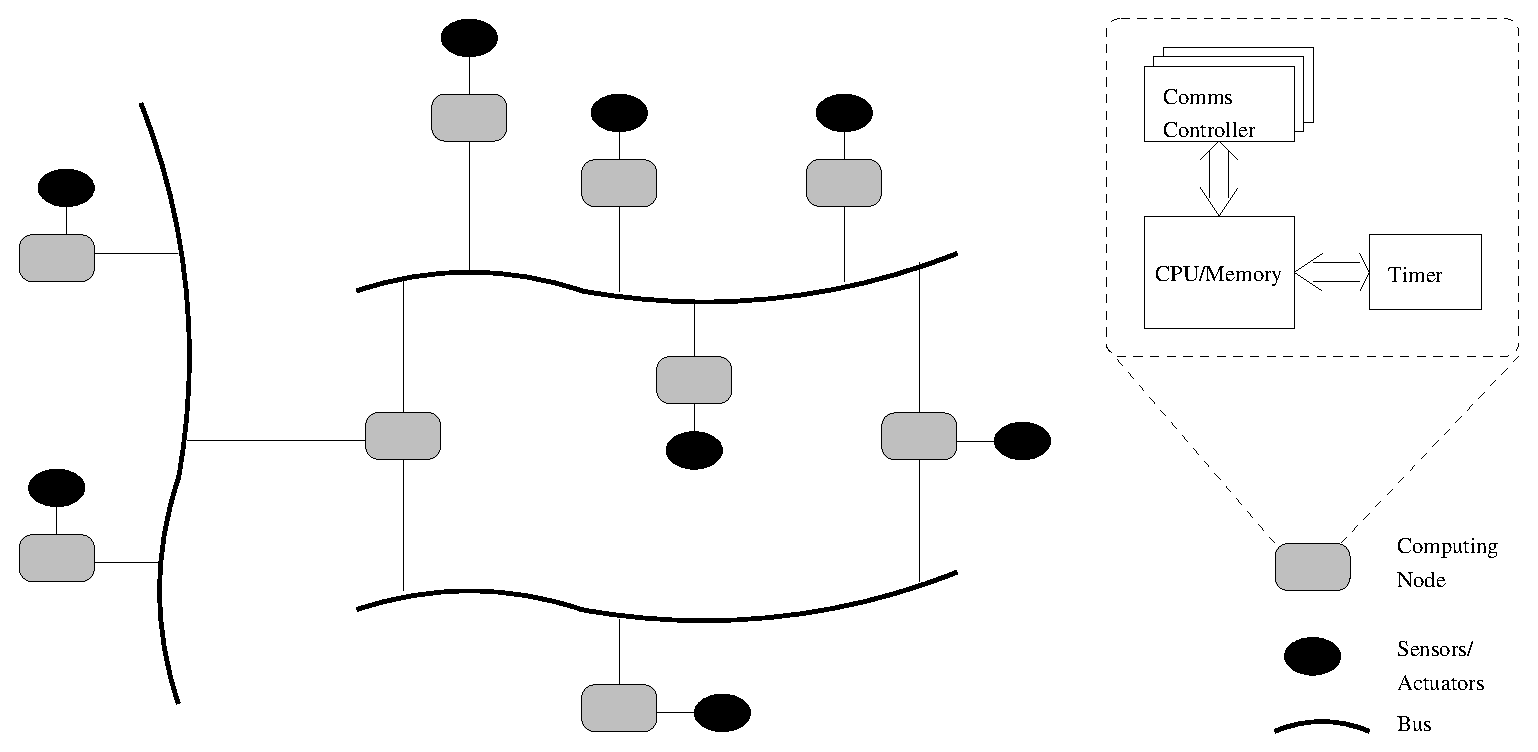
\includegraphics[width=.8\linewidth]{BCANDLE/sysmod.eps}
\end{center}
\caption{Control system model\label{fig:sysmod}}
\end{figure}
\begin{itemize}
\item Control is distributed over a set of {\em processes\/} which are
  statically allocated to computing nodes. 
\item A computing node consists
  of at least a central processing unit, which has access to some
  local memory, one or more communication controllers and a
  programmable timer.
\item Several processes may be allocated to a single computing node and 
  share its processing unit using some fixed scheduling policy. The
  approach taken in this work to the construction of timed models of
  control systems requires the choice of scheduling policy to be
  restricted to one which allows static calculation of computation
  response times: e.g. round-robin or cyclic executive. This allows
  the effects of scheduling to be accounted for when the model is
  constructed, without requiring the model to represent the scheduler
  explicitly. Future work will address how this constraint may be
  relaxed.
\item Processes communicate by using one or more communication channels 
  to send and receive broadcast messages. Each channel implements an
  abstraction of the CAN protocol, as discussed below.
\item Even processes which share a processor communicate by
  broadcasting messages, rather than by unconstrained access to shared
  memory, i.e., all processes communicate using (logically) a single
  mechanism, whether they share a computing node or not. This
  requirement simplifies the model and can be satisfied with
  acceptable efficiency in practice. For example, a CAN-style channel
  can be implemented using shared memory techniques such as condition
  variables~\cite{iso:96} or the mutable variables of Concurrent
  Haskell~\cite{pgf:96}. The latency of such a (pseudo-) channel is
  clearly different from that of a `real' CAN channel but can be
  modelled using the same techniques.
\item There is no interference between communications on \emph{different}
  channels, i.e. the transmission of a message on some channel $a$ has
  no effect on any other channel $b$, unless $a$ and $b$ are the same
  channel. This requirement can be satisfied simply by requiring that
  every node has a dedicated communication controller for each channel
  which it uses.
\item Each computing node may have access to a number of sensors
  and actuators which form part of the interface to the controlled
  system. In the case of multi-tasking, it is assumed that each sensor and
  actuator is accessed exclusively by a single process.
\end{itemize} 
  
In constructing a formal model of a system of the sort described
above, it is essential to abstract from some of the details, in order
to ensure that an analysis of the model is tractable. With this in
mind, the following features of an abstract model are identified:
\begin{itemize}
\item The \emph{data model} is an abstraction of the 
  set of local memories of the computing nodes. We adopt a single
  global mapping from data variables to data values and assume that
  locality is ensured by the syntax of a high-level modelling language.
\item The \emph{communication model} abstracts entirely from communication
  controllers and represents the communication channels only. It is
  assumed that communication channels operate without errors or
  failures. Also, the details of bit-level data transmission are
  abstracted by adopting the assumption that messages are transmitted
  atomically.
\item  The \emph{process model} represents the dynamic behaviour of
  processes, while abstracting from the allocation of processes to
  computing nodes, and from the scheduling policies adopted by
  multi-tasking nodes. We assume that an \emph{a priori} analysis 
  accounts for these factors in determining bounds on the completion
  times of computations. This assumption restricts the systems
  which can be modelled to those with simple cyclic scheduling policies,
  but seems essential for tractable analysis.
\end{itemize}
We present the formal description of each of these aspects of 
the system models in the following sections.

\section{The Data Model \label{sec:bcdata}}
Many approaches to the description of concurrent and real-time systems
have adopted the point of view that the data environment in which a
system acts can be either completely disregarded, or else encoded in
the system's behaviour in some way~\cite{mil:89,dav:93}.  This
assumption can simplify the semantic model and its analysis. However,
for many systems, the effects of data-dependent behaviour cannot be
ignored or abstracted from entirely, and the need to develop an
artificial encoding can be tiresome. Therefore we have chosen to
include an explicit model of (at least part of) the data environment in
our system models, and to employ appropriate abstractions 
in their analysis when it becomes clearer which properties of
the data environment are relevant to the system properties of
interest. A similar approach has been adopted in AORTA~\cite{bhkr:01}.

Unlike the LOTOS family of languages~\cite{lot:88,lot:98,lot:98a}, for
example, which give a very detailed description of a particular data
sub-language, \bcandle\ specifies only a minimal set of requirements which
a data language must satisfy. In principle, this allows the system
modeller to derive models from a variety of different data languages,
so long as they are well-defined with respect to the properties 
described below. For example, a high-level language such as B~\cite{abr:96},
a programming language such as Spark Ada~\cite{bar:96} or a simple guarded 
command language, as introduced in Chapter~\ref{chap:practice}, can
be used as the data language for \bcandle. Although some effort is 
required to establish the necessary semantic relations, it is rewarded
by the flexibility in the choice of language and the simplification
in the presentation of \bcandle. 

\subsection{Formal Definition}\label{ss:bcformaldata}
There are three kinds of syntactic object
relating to data which can occur in a \bcandle\ description: data variables,
operation names and predicate names (or guards). The necessary formal
definitions are introduced below.

Let $\Var$ be a finite set of data variables. Each variable $\xx \in
\Var$ takes its value from some non-empty, finite set of values
$\type(\xx) \subseteq \V$, where $\V$ is the set of data
values. We assume that $\V$ contains at least the distinguished value
$\undefined$, where $\undefined \notin \bigcup_{\xx \in \Var} \type(\xx)$, 
which is taken to be the ``undefined'' data value.
In modelling the behaviour of a system, the current valuation
of the data variables is given by a total function from variables to
values. The set of valuations is defined by:
\[ \valuation \defs \Var \fun \V \]
where for any $\val \in \valuation$ and $\xx \in \Var$, either
$\val(\xx) \in \type(\xx)$ or $\val(\xx) = \undefined$.

Data operations are modelled as relations on valuations. This allows
the use of non-deterministic operation specifications, which are often
useful in the construction of abstract system models. Let $\Op$ be a
finite set of operation names.  Each operation name $\op \in
\Op$ is interpreted by a total relation on valuations. The set of
operations is defined by:
\[ \operation \defs \valuation \rel \valuation \]
where it is required that for every operation $o$ and for every
valuation $\val$, there is at least one valuation to which $\val$ is
related by $o$, i.e. 
\[ \forall o \in \operation \such \dom(o) = \valuation\;.\]

Predicates on data are modelled simply as the sets of valuations which
satisfy them.  Let $\G$ be a finite set of predicate names.  Each
predicate name $\g \in \G$ is interpreted by the set of valuations
which satisfy it. The set of predicates is defined:
\[ \predicate \defs 2^\valuation \]

In defining a data environment $\D$ with respect to given sets of
data variables $\Var$, operation names $\Op$ and predicate names
$\G$, we say that $\D$ is a data environment \emph{over} $\Var, \Op$ and
$\G$, and denote the set of such environments by $\DataEnv{\Var,\Op,\G}$.
We can now formally define our notion of a data environment.
\begin{definition}[Data Environment]
Let $\Var$ be a finite set of variable names, $\Op$ a finite set of
operation names and $\G$ a finite set of predicate names. Let $\V$ be
the set of data values. A \emph{data environment} $\D$ over
$\Var, \Op$ and $\G$ is a tuple
\[ \D = (\type, \interpop, \interppred, \val) \]
where $(\type, \interpop, \interppred, \val) \in \DataEnv{\Var,\Op,\G}$ iff
\begin{itemize}
\item $\type : \Var \fun 2^\V$ is a total function, giving for each variable 
 $\xx \in \Var$, a non-empty, finite set of data values $\type(\xx)$
 ranged over by $\xx$;
\item $\interpop : \Op \fun \operation$ is a total function, giving for 
  each operation name $\op \in \Op$, an operation
  $\interpop(\op)$ which interprets it;
\item $\interppred : \G \fun \predicate$ is a total function, giving for each 
  predicate name $\g \in \G$, a predicate $\interppred(\g)$ which interprets 
  it;  
\item $\val : \Var \fun \V$ is a total function which, for each variable 
  $\xx \in \Var$, gives the current valuation of $\xx$, where $\val(\xx)
  \in \type(\xx)$ or $\val(\xx) = \undefined$.
\qed
\end{itemize}
\end{definition}

We assume that for a given \bcandle\ description, the interpretations
of the variable, operation and predicate names are fixed but that the
current valuation may change as the system evolves.

\begin{notation}
It is convenient to establish some notational conventions.  Let $\D =
(\type, \interpop, \interppred, \val)$ be a data environment. Let
$\xx,\yy \in \Var$ be data variables, and $\vv \in \V$ a data value.
\begin{itemize}
\item $\D.\type$, $\D.\interpop$, $\D.\interppred$ and
  $\D.\val$ denote $\type$, $\interpop$, $\interppred$ and $\val$,
  respectively. 
\item  $\D.\xx$ denotes the value $\val(\xx)$.
\item $\assign{\D}{\xx}{\vv}$ denotes the data environment 
  $\D' = (\type, \interpop, \interppred, \val')$ where 
  $\val'(\xx) = \vv$ and $\val'(\yy) = \val(\yy)$ for all $\yy \nsyneq \xx$ 
  ($\syneq$ denotes syntactic identity and $\nsyneq$ its negation).
\item $\D \goesdata{\op} \D'$ abbreviates the condition
  \[ (\val,\val') \in \interpop(\op) \land \D' = (\type, \interpop,
  \interppred, \val') \]

  We reserve the operation name $\ID$ and require that it is
  interpreted in any data environment by the operation
  $\interpop(\ID)$, where 
  \[
    \interpop(\ID) \defs \{(\val,\val)| \val \in \valuation\}
  \] 
  i.e., $\interpop(\ID)$ is the identity relation on valuations.
\item $\D \models \g$ abbreviates the condition $\val \in \interppred(\g)$.
  We write $\D \not \models \g$ for $\val \notin \interppred(\g)$. We
  reserve the predicate names $\True$ and $\False$ and require that
  $\forall \D \such \D \models \True \land \D \not \models \False$,
  i.e., $\True$ and $\False$ are interpreted in every data environment
  by $\interppred(\True)$ and $\interppred(\False)$, as follows:
  \begin{eqnarray*} \interppred(\True) & \defs & \valuation \\
  \interppred(\False) & \defs & \emptyset \end{eqnarray*}
\end{itemize}
\end{notation}
Let $\D_i = (\type_i, \interpop_i, \interppred_i, \val_i)$ for $i \in
\{1,2\}$ be two data environments. $\D_1$ and $\D_2$ are said to be 
\emph{compatible} iff $\type_1 = \type_2$, $\interpop_1 = \interpop_2$, and
$\interppred_1 = \interppred_2$. If $\D_1$ and $\D_2$ are compatible
data environments, and additionally $\val_1 = \val_2$, then $\D_1$ and
$\D_2$ are said to be \emph{equal}, denoted $\D_1 = \D_2$. Here it is
assumed that all component equalities are defined extensionally in the
usual way.
 
\section{The Network Model \label{sec:bcnetwork}}
A network model is an abstraction of a CAN network. It consists
of one or more broadcast channels, each implementing an abstraction of
the CAN protocol, as follows: 

\begin{itemize}
\item Each channel operates fault-free, i.e. without the need for error or
  overload frames.
\item A transmitting node only attempts to transmit its highest priority
message. (This requirement may seem obvious but in fact needs some
effort to satisfy when using some CAN controllers.) 
\item A node which has messages to transmit attempts to transmit its
highest priority message as soon as the channel is free. This implies
that each communication controller does not release the channel between
transmissions, i.e.  it enters a message for arbitration in every
arbitration phase if it has a message to transmit. This is important in
ensuring that lower priority messages cannot delay the transmission of
pending messages of higher priority by beginning transmission during a
``gap'' between message transmissions.
\item It is guaranteed that a message is ``simultaneously''
  accepted either by all nodes which are configured to accept it,
  or by none of them. There is no possibility of
  a ``partially successful'' transmission.
\item We assume that we can determine the point during the transmission
  of a message when a controller begins its acceptance test for the message.
  In normal operation, a controller which becomes configured to accept 
  messages  at any time before it begins its acceptance test, will accept all 
  messages which pass the test thereafter.
\end{itemize}

In the rest of this section, the structure of
channels and networks is considered first; this is followed by a 
consideration of network behaviour. 

\subsection{Structure}\label{ss:bcnetstructure}
A network is a collection of broadcast channels, each of which is capable of
transmitting messages from a single sending node to one or more
receiving nodes. Messages comprise a message identifier and a
data value. The identifier serves both to identify the type of
data contained in the message and also to give a priority to the
message for use in the arbitration of transmission collisions. The
remainder of this section expands and formalises these ideas.
\subsubsection{Messages}
The following example will be used throughout this section to illustrate
the ideas which are introduced.
\begin{exampleb}\label{xmpl:bcmessages}
Consider a simple system for monitoring the temperature of a liquid in
a chemical tank and the state of a heater which is used to regulate
the temperature. The monitoring system receives messages broadcast by
a pair of intelligent sensors, one giving the temperature of the
liquid and one giving the state of the heater.  Let $\I = \{HEATER,
TEMPERATURE\}$ be the set of message identifiers and $\V = \{ON, OFF\}
\cup \{-275 \upto 275\}$ be the set of data values. A message
consisting of message identifier $\ii$ and data value $\vv$ is denoted
$\ii.\vv$. Some possible messages are $HEATER.ON$ and
$TEMPERATURE.127$. The set of all possible messages is given by $\I
\cross \V$.  Notice, however, that some combinations of message
identifier and data value are not sensible, e.g., $HEATER.75$
and $TEMPERATURE.OFF$.
\qed
\end{exampleb}
 
Example~\ref{xmpl:bcmessages} suggests that it is helpful to identify the 
messages which a channel is allowed to transmit and leads us to the 
following definitions. 

\begin{definition}[Messages]
Let $\I$ be a finite set of message identifiers. Let $\V$ be the set
of data values. A set of \emph{messages} over $\I$ is any finite
subset $\M \subseteq \I \cross \V$.
\qed
\end{definition}

\begin{notation}
A \emph{message} $(\ii,\vv) \in \M$ is written $\ii.\vv$.
\end{notation}

\subsubsection{Message Priority}
Referring again to Example~\ref{xmpl:bcmessages}, it is clear that a
mechanism is needed to resolve the conflict which arises if the
temperature and heater sensors try to transmit their messages
simultaneously on the same channel. Such a conflict is resolved, as in
the CAN protocol, by assigning a priority ordering to the set of
message identifiers associated with the channel. Let $HEATER \pless
TEMPERATURE$ denote that $HEATER$ is a higher priority identifier than
$TEMPERATURE$.  Then, for example, if transmission of the messages
$HEATER.ON$ and \break $TEMPERATURE.127$ is initiated simultaneously, the
transmission of the higher priority message $HEATER.ON$ will succeed,
and the message \break $TEMPERATURE.127$ will compete again for the channel
when it next becomes idle.

\begin{definition}[Priority Ordering]
Let $\I$ be a set of message identifiers and $\V$ a set of data
values.  Let $\M \subseteq \I \cross \V$ be a set of messages.  A
\emph{priority ordering} is a strict total ordering $\pless\; : \I \rel \I$
on the message identifiers.  The reflexive
ordering $\pleq$\; is defined as usual: for all $\ii, \ii' \in \I$,
\[ \ii \pleq \ii' \iff \ii \pless \ii' \lor \ii = \ii'.\] 
A priority ordering on identifiers induces a partial ordering on the
message set $\M$. The derived ordering $\pless\; :
\M \rel \M$ satisfies for all $\mm,\mm' \in \M$,  
\[\mm \pless \mm' \iff \ii \pless \ii'\]
and the reflexive ordering $\pleq\; : \M \rel \M$ satisfies
\[\mm \pleq \mm' \iff \ii \pleq \ii'\]
where $\mm = \ii.\vv$ and $\mm' = \ii'.\vv'$, in each case. 
These orderings on messages are also referred to as priority orderings, and
the overloading is resolved by context.
\qed
\end{definition}

\subsubsection{Message Transmission}
Before transmission of a message can begin, it is required that no
other message is already being transmitted on the communication
channel; in this case, the channel is said to be \emph{free}. At some
time following the commencement of message transmission, all nodes
which are listening to the channel perform a test to determine whether
or not the message should be \emph{accepted}. This decision depends on
the identifier of the transmitted message. If the message identifier
matches a message identifier in the acceptance set of a node, then
the node accepts the message and the message data is made available
to processes residing on it, otherwise the node ignores the message.
It is assumed that all nodes perform the acceptance test
instantaneously at the same time. At some time after the acceptance
test, the channel becomes free again and is available to transmit
another message.

Three phases can be clearly identified in the transmission of a message.
The \emph{acceptance} phase is the point during the 
transmission of a message when listening nodes perform their acceptance
test. The \emph{pre-acceptance} phase extends from the start of transmission 
to the point of acceptance. The \emph{post-acceptance} phase extends from
the acceptance point to the instant at which the channel next becomes
free. 

The \emph{transmission latency} of a message is the time which passes
during the pre-acceptance and post-acceptance phases of message
transmission.  It is assumed that upper and lower bounds can be
determined for the pre-acceptance and post-acceptance latency of all
messages.
 
\begin{definition}[Transmission Latency]\label{def:bctransmissionlatency}
Let $\M$ be a set of messages.  A
\emph{transmission latency function for} $\M$ is a function $\latency
: \M \fun \TimeInf \cross \TimeInf \cross \TimeInf \cross \TimeInf$,
where $\latency(\mm) = (l,u,l',u')$ implies that $l \leq u$, $l' \leq
u'$ and that the lower and upper bounds on the pre- (resp. post-)
acceptance phase of the transmission of $\mm$ are given by $l$ and $u$
(resp. $l'$ and $u'$).

The derived functions $\dlb,\dub,\dlB,\duB : \M \fun \TimeInf$ satisfy
\begin{zed}
\forall \mm \in \M \such \dlb(\mm) = l \land \dub(\mm) = u \land 
 \dlB(\mm) = l' \land \duB(\mm) = u' \\
\t2 \iff \latency(\mm) = (l,u,l',u')
\end{zed} 
\qed
\end{definition}

\begin{notation}
The notation $\lb$ (resp. $\ub, \lB, \uB$) is used as an abbreviation
for $\dlb(\mm)$ (resp. $\dub(\mm), \dlB(\mm),
\duB(\mm)$) when $\mm$ is clear from the context.
\end{notation}

\begin{exampleb}
Refer again to Example~\ref{xmpl:bcmessages}. Let the transmission latency
function be defined as in Table~\ref{tab:bclatency}, 
\begin{table} 
\begin{center}
\begin{tabular}{|c||c|c|}
\hline \hline
& $HEATER.\_$ ($\mu$s) & $TEMPERATURE.\_$ ($\mu$s) \\
\hline
$\dlb$ & 43 & 55 \\
$\dub$ & 53 & 65 \\
$\dlB$ & 10 & 10 \\
$\duB$ & 12 & 12 \\
\hline \hline
\end{tabular}
\end{center}
\caption{Example of Transmission Latency Functions\label{tab:bclatency}}
\end{table}
where $HEATER.\_$ stands for the messages $HEATER.ON$ and $HEATER.OFF$
and $TEMPERATURE.\_$ stands for any message $TEMPERATURE.\vv$ with
$\vv \in \{-275 \upto 275\}$\footnote{Notice that here and throughout,
we make use of $\mathbf{\_}$ to denote an arbitrary value taken from
whatever set of values is appropriate in its context.}. Some example
interpretations are: the lower bound on the time taken to complete the
pre-acceptance phase of transmission of the message $HEATER.OFF$ is
$43\mu$s; the upper bound on the time taken to complete the
pre-acceptance phase of the transmission of the message
$TEMPERATURE.127$ is $65\mu$s; and the lower (resp. upper) bound on
the time taken to complete the post-acceptance phase of any message is
$10\mu$s (resp. $12\mu$s).
\qed
\end{exampleb}

The \emph{transmission status} of a channel identifies whether the
channel is free or is transmitting a message and, if transmitting a
message, whether it is in the pre-acceptance, acceptance or
post-acceptance phase.  If a channel is in its
pre-acceptance or post-acceptance phase, the bounds on the time to
completion of the phase are deemed to be part of its
transmission status, since they determine the time at which the
channel may next influence the behaviour of a system.  As time
passes, the bounds on the time to completion of a phase are reduced
equally until the lower bound becomes 0, after which the upper bound
may approach the lower bound until it too becomes 0.

\begin{definition}[Transmission Status]\label{def:bctransmissionstatus}
Let $\M$ be a set of messages and
$\latency : \M \fun \TimeInf \cross \TimeInf \cross \TimeInf \cross
\TimeInf$ a transmission latency function for $\M$. Let
$\{\FREE,\PRE,\ACCEPT,\POST\}$ be a set of distinct constant symbols.  
The set $\Status{\M,\latency}$ is defined:
\begin{eqnarray*}
\Status{\M,\latency} & \defs & \{\FREE\} \cup \PreAcceptance{\M,\latency}
                               \cup (\{\ACCEPT\} \cross \M) \\
                     & \cup  & \PostAcceptance{\M,\latency}
\end{eqnarray*}
where, for a message $m \in \M$, a lower bound $\ti_1 \in \TimeInf$ and 
an upper bound $\ti_2 \in \TimeInf$:
\begin{enumerate}
\item $(\PRE,\mm,\ti_1,\ti_2) \in \PreAcceptance{\M,\latency}$ iff
$\ti_1 \leq \dlb(\mm)$, $\ti_2 \leq \dub(\mm)$, and $\ti_2 - \ti_1 =
\dub(\mm) - \dlb(\mm)$ if $\ti_1 > 0$, otherwise $\ti_2 - \ti_1
\leq \dub(\mm) - \dlb(\mm)$; 
\item $(\POST,\mm,\ti_1,\ti_2) \in \PostAcceptance{\M,\latency}$ iff
$\ti_1 \leq \dlB(\mm)$, $\ti_2 \leq \duB(\mm)$, and $\ti_2 - \ti_1 =
\duB(\mm) - \dlB(\mm)$ if $\ti_1 > 0$, otherwise $\ti_2 - \ti_1
\leq \duB(\mm) - \dlB(\mm)$.
\qed
\end{enumerate}
\end{definition}
\begin{notation}
In the rest of the dissertation, the notation shown in
Figure~\ref{fig:transmissionstatus} is often used as a shorter and more
suggestive notation for transmission status.
\end{notation}

\begin{figure}
\begin{center}  
\begin{tabular}{|c|c|p{.6\linewidth}|}
\hline 
\bfseries Notation & \bfseries ASCII & \hfil \bfseries Transmission Status \hfil \\
\hline \hline
$\free$ & \verb!\/! & $\FREE$ \\ \hline
${}\preact{\ti_1,\ti_2}{\mm}$ & \verb!--t1,t2->m! &
                     $(\PRE,\mm,\ti_1,\ti_2)$, 
                     pre-acceptance phase of transmission of
                     message $\mm$ with bounds $\ti_1,\ti_2$ on time
                     to completion, $0 \leq \ti_1 \leq \lb$, 
                     $0 \leq \ti_2 \leq \ub$ \\ \hline 
${}\offers{\mm}$ & \verb!/\m! &
                    $(\ACCEPT,\mm)$,
                    acceptance point in transmission of $\mm$ \\ \hline
${}\postact{\ti_1,\ti_2}{\mm}$ & \verb!m--t1,t2->! &
                     $(\POST,\mm,\ti_1,\ti_2)$,
                     post-acceptance phase of transmission of
                     message $\mm$ with bounds $\ti_1,\ti_2$ on time to 
                     completion, $0 \leq \ti_1 \leq \lB$, 
                     $0 \leq \ti_2 \leq \uB$ \\ \hline
\end{tabular} 
\end{center}
\caption{Transmission Status Notation ($\mm \in \M$ and $\ti\protect_1, 
  \ti\protect_2 \in \TimeInf$)\label{fig:transmissionstatus}}
\end{figure}

\subsubsection{Message Queues}
If it is attempted to transmit a message on a channel which is not
free, the message must be stored and offered for transmission again
some time after the current transmission has finished. Since messages
succeed in their transmission attempts according to their priority, 
the storing of messages is modelled naturally as a priority ordered
queue. If an attempt is made to transmit a message $\mm$, whose
identifier is the same as that of another message $\mm'$ which is
already in the message queue, then $\mm$ replaces $\mm'$ in the queue
and $\mm'$ is lost forever, i.e. $\mm'$ is `overwritten' by $\mm$.
This represents the behaviour of most implementations of the CAN protocol.

\begin{definition}[Message Queue]\label{def:bcmessagequeue}
Let $\I$ be a finite set of message identifiers and $\V$ a set of data
values.  Let $\M \subseteq \I \cross \V$ be a set of messages and
$\pless$ a priority ordering for $\M$.  $\Queue{\M,\pless}$ is defined
to be the set of all sequences over the message set $\M$ which satisfy
the following two invariant properties:
\begin{eqnarray}
  \forall \mq \in \Queue{\M,\pless}; j,j' \in \dom \mq \such j < j' \implies 
     \mq(j) \pless \mq(j')
  \label{cond:bcpriorityordering} \\
   \forall \mq \in \Queue{\M,\pless}; \ii \in \I \such 
 \# \{\jj | \jj \in \dom \mq \land \mq(\jj) = \ii.\_\} \leq 1
 \label{cond:bconeidentifier}
\end{eqnarray}
i.e. All message queues preserve the priority ordering of messages 
  and contain at most one message with a given message identifier. 
\qed
\end{definition}

A corollary of property~\ref{cond:bconeidentifier} is that all message
queues are of finite length.
\begin{proposition}
Let $\I$ be a finite set of message identifiers and $\V$ a set of data
values.  Let $\M \subseteq \I \cross \V$ be a set of messages and
$\pless$ a priority ordering for $\M$. For all $\mq \in \Queue{\M,\pless}$,
$\mq$ is of finite length.
\end{proposition}
\begin{proof}
Immediate from property~\ref{cond:bconeidentifier} of
Definition~\ref{def:bcmessagequeue} and the fact that $\I$ is finite.
\end{proof}

\begin{notation}
An empty queue is denoted $\emq$. A queue with highest priority
message $\mm$ and remaining messages $\mq$ is written $\mm \cq
\mq$.
\end{notation}

The queueing of a message is modelled by the following operation.
\begin{definition}[Message Queue Insertion]
Let $\I$ be a set of message identifiers and $\V$ a set of data
values.  Let $\M \subseteq \I \cross \V$ be a set of messages and
$\pless$ a priority ordering for $\M$. The insertion operator $\iq :
\Queue{\M,\pless} \cross M \fun \Queue{\M,\pless}$ is defined:
\[
\mq \iq \ii.\vv =
\begin{cases}
\la \ii.\vv \ra & ,\IF \mq = \emq \\
\ii.\vv \cq \mq' & ,\IF \mq = \ii.\_ \cq \mq' \\
\ii.\vv \cq \mm \cq \mq' & ,\IF \mq = \mm \cq \mq' \land \ii.\vv \pless \mm \\
\mm \cq (\mq' \iq \ii.\vv) & ,\IF \mq = \mm \cq \mq' \land \mm \pless \ii.\vv
\end{cases}
\]
\qed
\end{definition}
It is easy to show that $\iq$ preserves the message queue invariants.
\begin{proposition}
Let $\M$ be a set of messages and
$\pless$ a priority ordering for $\M$.  For all $\mq \in
\Queue{\M,\pless}$ and all $\mm \in \M$, $\mq \iq
\mm$ satisfies properties~\ref{cond:bcpriorityordering}
and~\ref{cond:bconeidentifier} of Definition~\ref{def:bcmessagequeue}.
\end{proposition}
\begin{proof}
Induction on the length of $\mq$.
\end{proof}

\subsubsection{Channels}
All of the prerequisites for the definition of communication channels
have now been introduced.

\begin{definition}[Channel]
Let $\I$ be a set of message identifiers. Let $\V$ be the set of data
values. A \emph{channel} over $\I$ is a tuple
$(\M,\pless,\latency,\ss,\mq)$. The set of channels over $\I$ is
denoted $\Channel{\I}$, and $(\M,\pless,\latency,\ss,\mq) \in
\Channel{\I}$ iff
\begin{itemize}
\item $\M \subseteq \I \cross \V$ is a set of messages,
\item $\pless : \I \rel \I$ is a priority ordering,
\item $\latency : \M \fun \TimeInf \cross \TimeInf \cross \TimeInf \cross 
  \TimeInf$ is a transmission latency function, 
\item $\ss : \Status{\M,\latency}$ is a transmission status
\item $\mq : \Queue{\M,\pless}$ is a message queue
\qed
\end{itemize}
\end{definition}

Let $(\M,\pless,\latency,\ss,\mq)$ be a channel. It is
assumed that $\M$, $\pless$ and $\latency$ are \emph{static}, i.e.,
defined at system initialisation and unchanging thereafter. On the
other hand, $\ss$ and $\mq$ are used to model the current transmission
status and message queue of a channel as a system evolves, and are
therefore \emph{dynamic}.

The variables $\channel, \channel', \channel_1$ etc. are used to range
over channels. Let $\channel_i =
(\M_i, \pless_i, \\ \latency_i, \ss_i, \mq_i)$ be two channels. $\channel_1$
and $\channel_2$ are said to be \emph{equal}, denoted $\channel_1 =
\channel_2$, iff $M_1 = M_2$, $\pless_1\; =\; \pless_2$, $\latency_1 =
\latency_2$, $\ss_1 = \ss_2$ and $\mq_1 = \mq_2$, where the component
equalities are defined extensionally as usual.

\subsubsection{Networks}
A network is a collection of channels in which each channel is associated
with its own unique identifier.

\begin{definition}[Network]
Let $\K$ be a finite set of channel identifiers and $\I$ a finite
set of message identifiers.
A \emph{network} $\N$ over $\K$ and $\I$ is a mapping 
$\N : \K \fun \Channel{\I}$. The set of networks over
$\K$ and $\I$ is denoted $\Network{\K,\I}$, where 
$\Network{\K,\I} \defs \K \fun \Channel{\I}$.
\qed
\end{definition}

\begin{notation}
Let $\K$ be a set of channel identifiers and $\N$ a network over $\K$.
Let $\kk \in \K$ be a channel identifier. We write $\N_\kk$ for the function 
application $\N(\kk)$, i.e. $\N_\kk$ denotes the channel associated with
the identifier $\kk$ in the network $\N$.
\end{notation}
Network equality is defined extensionally as usual.
 
\subsection{Behaviour}\label{ss:bcnetbehaviour}
Each channel in a network can act independently by making a
discrete change in its transmission status or its message
queue. Alternatively, the state of the whole network may be affected
as time progresses. We consider first the modelling of discrete state
changes.

When a channel $\channel$ makes a discrete change, it gives
rise to a new network state in which $\channel$ is in its new state
and the state of all the other channels is the same as before. It is
convenient to introduce an operator which models the effect on a
network of a change of state in a single channel.
\begin{definition}[Network Update]
Let $\K$ be a set of channel identifiers and $\I$ a set of message
identifiers. Let $\N \in \Network{\K,\I}$ be a network.  
Let $\channel \in \Channel{\I}$ be a channel. The
notation $\assign{\N}{\kk}{\channel}$ denotes the network $\N'$,
where $\N'_\kk = \channel$ and $\N'_{\kk'} = \N_{\kk'}$, for all $\kk'
\in \K \setminus \{\kk\}$.
\qed
\end{definition}

Network behaviour is modelled by a relation ${}\goesn{}{} \subseteq
\Network{} \cross (\NetLabels \cup \Time) \cross \Network{}$ which represents
possible changes in network state.  As usual, $(\N,\nort,\N') \in
{}\goesn{}{}$ is written $\N \goesn{\nort} \N'$ and represents a
change of state from $\N$ to $\N'$ annotated with the label $\nort$
which ranges over $\NetLabels \cup \Time$. $\NetLabels$ is the set of
network action labels which are used to annotate discrete state
changes. Elements of $\Time$ are used to annotate state changes due to
the passage of time.
\begin{definition}[Network Action Labels]
Let $\V$ be the set of data values.
The set $\NetLabels$ of \emph{network action labels} over $\K$ and
$\I$ is defined by:
\[
\begin{array}{lcll}
\NetLabels & \defs & \{\kk\preact{}\ii.\vv | \kk \in \K \land \ii \in \I \land \vv \in \V\} & \quad \text{(* pre-acceptance *)} \\
& \cup & \{\kk\offers\ii.\vv | \kk \in \K \land \ii \in \I \land \vv
\in \V\} & \quad \text{(* acceptance *)} \\ 
& \cup & \{\postact{}{\ii.\vv}\kk | \kk \in \K \land \ii
\in \I \land \vv \in \V\} & \quad \text{(* post-acceptance *)} \\ 
& \cup & \{\kk\free | \kk \in \K\} & \quad \text{(* free *)} 
\end{array}
\]
where $\K$ and $\I$ are sets of channel identifiers and message
identifiers, respectively.
\qed
\end{definition}


\begin{notation}
In describing the behaviour of a network, it is often convenient to
mention only the dynamic components of each network channel. 
For example, the channel $(\M,\pless,\latency,\ss,\mq)$ may be written
$(\ss,\mq)$. The static components ($\M,\pless$ and $\latency$)
are inferred from the context.
\end{notation}

The relation ${}\goesn{}{}$ is given by a set of Plotkin-style inference
rules, as introduced below.

\subsubsection{Pre-Acceptance}
A channel which has a non-empty queue of pending messages, and whose
transmission status is free, starts transmission of its highest
priority message. The transmitted message $\mm$ is removed from the pending
queue and the transmission status of the channel shows that it is in
the pre-acceptance phase of transmission of $\mm$. The lower and upper
bounds on the time to completion of the pre-acceptance phase are given
by $\dlb(\mm)$ and $\dub(\mm)$, respectively. This is expressed 
formally by the rule \textbf{N.1} below:
\[\rpre\]

\subsubsection{Acceptance}
When the lower bound on the time to completion of the pre-acceptance
phase of the transmission of the message $\mm$ becomes 0, a channel
can change state to the acceptance phase of the transmission of $\mm$.
This is expressed formally by the rule \textbf{N.2} below:
\[\raccpt\]

\subsubsection{Post-Acceptance}
A channel in the acceptance phase of the transmission of a message
$\mm$ can enter the post-acceptance phase, whose bounds on time to
completion are given by $\dlB(\mm)$ and $\duB(\mm)$. This is expressed
formally by the rule \textbf{N.3} below:
\[\rpost\]

\subsubsection{Free}
When the lower bound on the time to completion of the post-acceptance
phase of the transmission of the message $\mm$ becomes 0, a channel
can change its state to free. This is expressed formally by the rule
\textbf{N.4} below:
\[\rfree\]

\subsubsection{Time Progress}
In order for time progress to be possible for a network $\N$, it must
be possible for \emph{all} channels in $\N$; the rate of progress is
the same in all channels.  A free channel allows time to pass
indefinitely if its message queue is empty, but must begin
transmission of its highest priority message without delay
otherwise. Similarly, a channel at its acceptance point does not allow
time to pass. Passage of time in the pre-acceptance and
post-acceptance phases of message transmission is bounded by the time
to completion of the phase. We define a function $\tcp$ which
determines, for any given channel, the maximum amount of time that can
pass before the channel must make a discrete state change.
\begin{definition}[Time Progress]\label{def:bctcp}
Let $\channel$ be a channel. The maximum time progress allowed for
$\channel$ is given by $\tcp(\channel)$, where
\begin{alignat*}{3}
\tcp(\free,\langle\rangle) & \defs \infinity & \quad \tcp(\free,\_:\_) & \defs  0 & \quad \tcp(\preact{\_,\ti}{\_},\_) & \defs  \ti \\ 
\tcp(\offers{\_},\_) & \defs  0  & \quad \tcp(\postact{\_,\ti}{\_},\_) & \defs  \ti && \\
\end{alignat*}
Let $\K$ be a set of channel identifiers and $\N$ a network over $\K$. 
The maximum time progress allowed for $\N$ is
given by $\tcp(\N)$, which is defined by
\[
\tcp(\N) \defs \min\{\tcp(\N_\kk) | \kk \in \K\}
\]
where $\min S$ returns the minimum of the finite, ordered set $S$.
\qed
\end{definition}

When time passes, the state of the network changes accordingly. We use
the notation $\channel + \ti$ (resp. $\N + \ti$) to denote the state of the 
channel $\channel$ (resp. network $\N$) after the passage of $\ti$ units of 
time.
\begin{definition}[Effect of time progress: Channels]\label{def:bcprogresschannels}
Let $\channel$ be a channel. Let $\ti \in \Time$. The state of the
channel $\channel$ after the progress of $\ti$ units of time is denoted
$\channel + \ti$, where $\channel + \ti$ is defined by:
\begin{eqnarray*}
(\free,\langle\rangle) + \ti & \defs & (\free,\langle\rangle) \\
(\free,\mm:\mq) + \ti & \defs & \ite{\ti=0}{(\free,\mm:\mq)}{\undefined} \\
(\preact{\ti_1,\ti_2}{\mm},\mq) + \ti & \defs & \ite{\ti \leq \ti_2}{(\preact{\ti_1\nmin \ti,\ti_2\nmin \ti}{\mm},\mq)}{\undefined} \\
(\offers{\mm},\mq) + \ti & \defs & \ite{\ti=0}{(\offers{\mm},\mq)}{\undefined} \\
(\postact{\ti_1,\ti_2}{\mm},\mq) + \ti & \defs & \ite{\ti \leq \ti_2}{(\postact{\ti_1\nmin \ti,\ti_2\nmin \ti}{\mm},\mq)}{\undefined} 
\end{eqnarray*}
where $\channel + \ti = \undefined$ is interpreted to mean that the result
is not a well-defined channel. 
\qed
\end{definition}

\begin{proposition}\label{prop:bcprogresschannels}
Let $\channel$ be a channel. Then, $\channel + 0 = \channel$.
\end{proposition}
\begin{proof}
Immediate from Definition~\ref{def:bcprogresschannels}.
\end{proof}

\begin{definition}[Effect of time progress: Networks]
\label{def:bcprogressnets}
Let $\K$ be a set of channel identifiers and 
$\N$ a network over $\K$. Let $\ti \in \Time$. The state of the network $\N$ 
after the progress of $\ti$ units of time is denoted by $\N + \ti$, where
\[
\N + \ti \quad \defs \quad 
\begin{cases}
\{\kk \mapsto (\N_\kk + \ti) | \kk \in \K\}, & \quad \forall \kk \in \K \such \N_\kk + \ti \neq \undefined  \\
\undefined, & \quad\text{otherwise}
\end{cases}
\]
where $\N + \ti = \undefined$ is interpreted to mean that the result is
not a well-defined network.
\qed
\end{definition}

\begin{proposition}\label{prop:bcprogressnets}
Let $\N$ be a network. Then, $\N + 0 = \N$.
\end{proposition}
\begin{proof}
By Definition~\ref{def:bcprogressnets} and Proposition~\ref{prop:bcprogresschannels}.
\end{proof}

\begin{proposition}\label{prop:bcnetdefinedaftertime}
For any network $\N$ and time $\ti \in \Time$, if $0 \leq \ti \leq \tcp(\N)$
then $\N + \ti$ is well-defined, i.e., $\N + \ti \neq \undefined$.
\end{proposition}
\begin{proof}
Immediate from definitions~\ref{def:bctcp} and~\ref{def:bcprogressnets}.
\end{proof} 

If all channels in a network $\N$ can allow time to progress by $\ti$
time units, then $\N$ can allow time to progress by $\ti$ time units,
changing state to become $\N + \ti$. This is expressed formally by the
rule \textbf{N.5} below:
\[\rtime\]

\begin{proposition}\label{prop:bcnetgoesbyzero}
Let $\N$ be a network. Then, $\N \goesn{0} \N$.
\end{proposition}
\begin{proof}
Immediate from N.5, Proposition~\ref{prop:bcprogressnets} and 
Definition~\ref{def:bctcp}.
\end{proof}

\subsubsection{Summary}
For ease of reference, we summarise the discussion of network 
behaviour by giving the following definition:
\begin{definition}[Network Behaviour]\label{def:bcnetsemantics}
Let $\V$ be the set of data values.  Let $\K$ and $\I$ be sets of
channel identifiers and message identifiers, respectively. Let
$\NetLabels$ be the set of action labels over $\K$ and $\I$. The
\emph{network behaviour relation} ${}\goesn{}{} \subseteq
\Network{\K,\I} \cross (\NetLabels
\cup \Time) \cross \Network{\K,\I}$ is given by the rules of 
Figure~\ref{fig:nettrans}, where for all $\N, \N' \in \Network{}$ and
$\nort \in \NetLabels \cup \Time$, $\N \goesn{\nort} \N'$ iff this can be
inferred from the rules {\bf N.1} -- {\bf N.5}.
\qed
\end{definition}
\begin{figure*}
\begin{minipage}{\linewidth}
\small%\scriptsize
\setlength{\extrarowheight}{5ex}
\begin{center}
\begin{tabular}{|ll|}
\hline
\multicolumn{2}{|c|}{\rpre} \\
\multicolumn{2}{|c|}{\raccpt} \\
\multicolumn{2}{|c|}{\rpost} \\
\multicolumn{2}{|c|}{\rfree} \\
\multicolumn{2}{|c|}{\rtime} \\
\hline
\end{tabular}
\end{center}
\end{minipage}
\caption{Rules for Network Behaviour\label{fig:nettrans}}
\end{figure*}

It is clear that ${}\goesn{}{}$ is well-behaved in that, if 
$\N \goesn{\nort} \N'$, then $\N'$ is a well-defined network and all
of the static components are the same in $\N$ and $\N'$.  
\begin{proposition}
Let $\K$ be a set of channel identifiers and $\N$ a network over $\K$.
If $\N \goesn{\nort} \N'$, then $\N' \neq \undefined$, and, for any
channel identifier $\kk$, where $\N_\kk =
(\M, \pless, \latency, \ss, \mq)$ and $\N'_\kk =$
$(\M', \pless', \latency', \ss', \mq')$, the following properties hold:
\begin{enumerate}
\item $\M = \M'$, ${}\pless{} = {}\pless'{}$ and $\latency = \latency'$;
\item $\ss' \in \Status{\M,\latency}$
\item $\mq' \in \Queue{\M,\pless}$
\end{enumerate}
\end{proposition}
\begin{proof}
The proofs of all properties follow directly from case analysis of the
rules \textbf{N.1} -- \textbf{N.5} by which $\N \goesn{\nort} \N'$ is
inferred.  That $\N' \neq \undefined$ is immediate from \textbf{N.5}
and Proposition~\ref{prop:bcnetdefinedaftertime}. Properties~1--3
follow from \textbf{N.1} -- \textbf{N.5} and
Definitions~\ref{def:bctransmissionstatus} and~\ref{def:bcmessagequeue}.
\end{proof}

\subsubsection{Example of network behaviour}
We now give an example of the possible behaviour of a simple
network.
\begin{exampleb}
Consider a network consisting of a single channel which
can transmit messages of type $temperature$ or of type $pressure$. Assume
that the values transmitted are abstractions of actual sensor
readings, where $0$ represents a reading in the low range, $1$ a
reading in the normal range, and $2$ a reading in the high range. 
The network can be defined as follows.
  
The message identifiers are given by the set $\I = \{temperature, pressure\}$, 
with priority order ${}\pless{}$ given by $temperature \pless
pressure$. The set of data values is $\V = \{0,1,2\}$ and the set of messages is $\M = \I \cross \V$. There is a single channel identifier given
by the set $\K = \{\kk\}$.
The function $\latency$ specifies transmission latencies in $\mu$secs, as
follows:
\begin{center}
\begin{tabular}{|>{$}l<{$}|>{$}c<{$}>{$}c<{$}|}
\hline
             & temperature.\_ & pressure.\_ \\
\hline
\dlb         &    43       &    32    \\
\dub         &    53       &    42    \\
\dlB         &    10       &    10    \\
\duB         &    12       &    12    \\
\hline
\end{tabular}
\end{center}

The network is $\N = \{\kk \mapsto (\M, \pless, \latency, \free, 
\langle temperature.1, pressure.0\rangle)\}$. Notice that we are assuming 
that the messages $temperature.1$ and $pressure.0$ have already been placed 
in the message queue of $\kk$. 

Now a possible trace of the network behaviour from this initial state is given
in Figure~\ref{fig:bcnetbehaviour}.
\qed
\end{exampleb}
The behaviour given in this example is very simple,
since messages are transmitted but not received. How a network 
interacts with receiving processes is considered in the following section.

\begin{figure}
\begin{center}
\begin{math}
\begin{array}{lll}
(\free,\langle temperature.1,pressure.0 \rangle) 
& \goesn{\kk\preact{}temperature.1} & (N.1) \\
(\preact{43,53}{temperature.1},\langle pressure.0 \rangle)
& \goesn{47} & (N.5) \\
(\preact{0,6}{temperature.1},\langle pressure.0 \rangle)
& \goesn{\kk\offers{temperature.1}} & (N.2) \\
(\offers{temperature.1},\langle pressure.0 \rangle)
& \goesn{\postact{}{temperature.1}\kk} & (N.3) \\
(\postact{10,12}{temperature.1},\langle pressure.0 \rangle)
& \goesn{12} & (N.5) \\
(\postact{0,0}{temperature.1},\langle pressure.0 \rangle)
& \goesn{\kk\free} & (N.4) \\
(\free,\langle pressure.0 \rangle)
& \goesn{\kk\preact{}pressure.0} & (N.1) \\
(\preact{32,42}{pressure.0},\emq)
& \goesn{32} & (N.5) \\
(\preact{0,10}{pressure.0},\emq)
& \goesn{\kk\offers{pressure.0}} & (N.2) \\
(\offers{pressure.0},\emq)
& \goesn{\postact{}{pressure.0}\kk} & (N.3) \\
(\postact{10,12}{pressure.0},\emq)
& \goesn{11} & (N.5) \\
(\postact{0,1}{pressure.0},\emq)
& \goesn{\kk\free} & (N.4) \\
(\free,\emq)
& \goesn{5} & (N.5) \\
(\free,\emq)
& \goesn{2} & (N.5) \\
(\free,\emq)
& \goesn{500} & (N.5) \\
\vdots
\end{array}
\end{math}
\end{center}
\caption{Example of network behaviour\label{fig:bcnetbehaviour}}
\end{figure}

\section{The Process Model \label{sec:bcprocesses}}
We use a simple process language to describe the behaviour of
processes.  In choosing the operators of the language, we have been
concerned to identify a small set which allows us to express naturally
the behavioural models in which we are interested, while allowing the
definition of a timed transition semantics in a direct manner. The
syntax and informal semantics of the language are presented in this
section. Section~\ref{sec:bcformalmodel} gives a formal semantics
and the work of the numerous researchers which has influenced the
language design is discussed in~\Sec\ref{sec:bcconc}.
 
\subsection{Syntax}
\begin{definition}[Process terms]\label{def:bcsyntax}
Let $\K$ and $\I$ be finite sets of channel identifiers and message
identifiers, respectively. Let $\Var$ be a finite set of data
variables, $\Op$ a finite set of operation names and $\G$ a finite set
of predicate names. Finally, let $\TimeInf$ be the time domain and
$\XX$ a countable set of process variables.  The set of \emph{process
terms} over $\K, \I, \Var, \Op$ and $\G$ is denoted 
$\ProcO{\K,\I,\Var,\Op,\G}$, and is defined inductively by:
\begin{center}
\begin{tabular}{>$l<$>$c<$>$l<$>$l<$}
P  & ::= &  \kk!\ii.\xx & \text{ (* send broadcast message *) } \\
   & |   &  \kk?\ii.\xx & \text{ (* receive broadcast message *) } \\
   & |   &  [\op : t_1, t_2] & \text{ (* time-bounded computation *) } \\
   & |   &  \g \guard P  & \text{ (* data guard *) } \\
   & |   & \P \seqcomp \P & \text{ (* sequential composition *) } \\
   & |   & \P \choice \P  & \text{ (* non-deterministic choice *) } \\
   & |   & \P \interrupt \P & \text{ (* interrupt *) } \\
   & |   & \P \parallel \P  & \text{ (* parallel composition *) } \\
   & |   & \rec X.\P & \text{ (* recursion *) } \\
   & |   & X & \text{ (* process variable *) } 
\end{tabular}
\end{center}
where $\kk \in \K$, $\ii \in \I$, $\xx \in \Var$, $\op \in \Op$, $\g \in \G$, 
$X \in \XX$ and $t_1 \leq t_2 \in \TimeInf$. 
\qed
\end{definition}

\begin{notation}
The subscript is dropped from $\ProcO{\K,\I,\Var,\Op,\G}$ if it is not
relevant or can be inferred from the context.
\end{notation}

Terms of the form $\kk!\ii.\xx$, $\kk?\ii.\xx$ and $[\op : t_1, t_2]$
are called \emph{basic terms}. We use variables $\basic, \basic_1,
\basic_2 \ldots$ to range over basic terms.
The precedence of the operators, from high to low is: $\guard,
\seqcomp, \choice, \interrupt, \rec, \parallel$. 
We use a number of syntactic abbreviations:
\begin{alignat*}{3}
[\op : \ti_1] & \defs [\op : \ti_1, \ti_1] & \qquad
[\ti_1] & \defs [\ID : \ti_1] & \qquad 
[\ti_1, \ti_2] & \defs [\ID : \ti_1, \ti_2] \\
\idle & \defs [\ID : \infinity] & \qquad 
\donothing & \defs [\ID : 0] && \\
\end{alignat*}
\emph{Free} and \emph{bound} variables are defined as usual.
\begin{definition}[Free and bound variables]
\mbox{\strut} \\
Let $P \in \ProcO{}$ and $\genop\, \in
\{\sq,\choice,\interrupt,\parallel\}$.  The \emph{free (process)
variables} and \emph{bound (process) variables} of $P$ are given by
$\fv(P)$ and $\bv(P)$ respectively, which are defined as the least
sets satisfying:
\begin{small}
\begin{alignat*}{2}
\fv(\kk!\ii.\xx) & = \emptyset & 
\bv(\kk!\ii.\xx) & = \emptyset \\ 
\fv(\kk?\ii.\xx) & = \emptyset & 
\bv(\kk?\ii.\xx) & = \emptyset \\ 
\fv([\op:t_1,t_2]) & = \emptyset & 
\bv([\op:t_1,t_2]) & = \emptyset \\ 
\fv(\g \guard \P) & = \fv(\P) &
\bv(\g \guard \P) & = \bv(\P) \\
\fv(X) & = \{X\} & 
\bv(X) & = \emptyset \\ 
\fv(\rec X.\P) & = \fv(\P) \setminus \{X\} &
\bv(\rec X.\P) & = \bv(\P) \cup \{X\} \\
\fv(\P \genop \Q) & = \fv(\P) \cup \fv(\Q) & 
\bv(\P \genop \Q) & = \bv(\P) \cup \bv(\Q) \quad\quad\quad\quad \qed
\end{alignat*}
\end{small}
\end{definition}

\begin{definition}[Closed term]
For any $\P \in \ProcO{}$, $\P$ is a \emph{closed} term if $\fv(\P) =
\emptyset$.
\qed
\end{definition}

The use of sequential composition as a basic operator, rather than
action prefix, requires some care in the definition of guarded terms.
\begin{definition}[Guarding, Guarded process variable, Guarded term]
Any basic term $\basic \in \ProcO{}$ is \emph{guarding}. A term
of the form $\P_1 \sq \P_2$ or $\P_1 \parallel \P_2$ is \emph{guarding}
if $\P_1$ is guarding or $\P_2$ is guarding. A term of the form 
$\P_1 \choice \P_2$ or $\P_1 \interrupt \P_2$ is \emph{guarding} if
$\P_1$ and $\P_2$ are guarding. A term of the form $\rec X.\P$ is
\emph{guarding} if $\P$ is guarding.

Let $\P \in \ProcO{}$ be a term containing one or more \emph{occurrences}
of a variable $X \in \XX$.
An occurrence of $X$ is \emph{guarded} in $\P$ if $\P$ has a subterm of
the form $\P_1 \sq \P_2$ where the occurrence of $X$ is contained in
$\P_2$ and $\P_1$ is guarding. Otherwise this occurrence
of $X$ is \emph{unguarded} in $\P$. A process variable $X$ is \emph{guarded}
in a term $\P$ if every occurrence of $X$ is guarded in $\P$. A term $\P$
is \emph{guarded} if all of its process variables are guarded in $\P$.
\qed
\end{definition}

\begin{definition}[Closed, guarded terms]
The set $\Proc{} \subset \ProcO{}$ is defined to be the set of 
closed, guarded terms in $\ProcO{}$.
\qed
\end{definition}

\subsubsection{Equational Presentation}
In practice, the use of the recursion operator $\rec X.\P$ is often
inconvenient and the use of a set of mutually recursive equations is
preferable.  We will use whatever form is more convenient in its
context and regard a term defined using a set of simultaneous
equations as denoting its corresponding term given in terms of the recursion
operator.
\begin{definition}
Let $\Equ$ be a finite set of equations $\{X_1 \defs P_1, X_2 \defs P_2,
\ldots, X_n \defs P_n\}$ where $\bigcup_{i\in\{1\upto n\}} \fv(P_i)
\subseteq \{X_1,\ldots,X_n\}$. Let $\P$ be a process term, $\fv(\P)
\subseteq \{X_1,\upto,X_n\}$. Then, the process term
corresponding to $\P$ is given by the normal form of $\P^\Equ$ under the
rewrite relation $\goesrw$, defined by:
\[
\begin{array}{llllll}
\multicolumn{6}{l}{
X^\Equ \goesrw \begin{cases} 
           \rec X.(P^{\Equ \setminus \{X \defs P\}}) 
              \quad\text{if $(X \defs P) \in \Equ$,} \\ 
           X  \quad \text{otherwise}
         \end{cases} } \\   
  (\kk!\ii.\xx)^\Equ & \goesrw & \kk!\ii.\xx &
  (\kk?\ii.\xx)^\Equ & \goesrw & \kk?\ii.\xx \\ 
  ([\op:t_1,t_2])^\Equ & \goesrw & [\op:t_1,t_2] & (\g \guard P)^\Equ & \goesrw & \g \guard (P)^\Equ \\  
  (P \seqcomp Q)^\Equ & \goesrw & (P)^\Equ \seqcomp (Q)^\Equ & (P \choice Q)^\Equ
  & \goesrw & (P)^\Equ \choice (Q)^\Equ \\ 
  (P \interrupt Q)^\Equ & \goesrw & (P)^\Equ \interrupt (Q)^\Equ & (P \parallel Q)^\Equ & \goesrw & (P)^\Equ \parallel (Q)^\Equ
\end{array}
\]
\qed
\end{definition}

\pagebreak
\begin{exampleb}
Consider the equational presentation
\begin{verbatim}
      A
      where
      A = [a:1] ; B
      B = [b:1] ; A
\end{verbatim}
Let $E_A \defs \{A \defs [a:1] \sq B\}$, $E_B \defs \{B \defs [b:1] \sq A\}$,
and $E \defs E_A \cup E_B$.

Then, with respect to $E$, $A$ is taken to stand for the term
\begin{eqnarray*}
A^E & \goesrw & \rec A . ([a:1] \sq B)^{E_B} \\
    & \goesrw & \rec A . [a:1]^{E_B} \sq B^{E_B} \\
    & \goesrw & \rec A . [a:1] \sq B^{E_B} \\
    & \goesrw & \rec A . [a:1] \sq \rec B . ([b:1] \sq A)^\emptyset \\
    & \goesrw & \rec A . [a:1] \sq \rec B . [b:1]^\emptyset \sq A^\emptyset \\
    & \goesrw & \rec A . [a:1] \sq \rec B . [b:1] \sq A^\emptyset \\
    & \goesrw & \rec A . [a:1] \sq \rec B . [b:1] \sq A
\end{eqnarray*} 
\qed
\end{exampleb}

\subsection{Informal Semantics}
Each process term represents a potential process which, when given a
\emph{context} (i.e., a network and a data environment), is capable of
exhibiting some behaviour. We give an informal introduction to the
behaviour of process terms in the remainder of this section. The
formal semantics is deferred to~\Sec\ref{sec:bcformalmodel}.

\begin{trivlist}
\item[{\bf Send}]
The term, $\kk!\ii.\xx$, denotes a process which causes a
message to be queued for transmission on channel $\kk$. The message
consists of the message identifier, $\ii$, and the data value 
associated with the variable, $\xx$. Sending is asynchronous. The
process $\kk!\ii.\xx$ cannot be delayed. It causes its message
to be queued instantaneously and terminates immediately.

\item[{\bf Receive}]
$\kk?\ii.\xx$ is a process which waits to accept a message from
channel $\kk$. It will only accept a message with the identifier
$\ii$. It ignores messages with any other identifier, simply
allowing time to pass and other network activity to occur.  When an
$\ii$-message reaches its acceptance point during transmission on
channel $\kk$, then $\kk?\ii.\xx$ must accept the message instantly,
causing the data variable $\xx$ to become associated with the
message's data value.  $\kk?\ii.\xx$ then terminates immediately.

\item[{\bf Compute}]
$[\op : t_1, t_2]$ is a process which transforms the data state
according to the specification of the operation $\op$. It begins 
execution immediately and is guaranteed to terminate no later
(resp. no sooner) than $t_2$ (resp. $t_1$) time units after it has 
started. The specified change to the data state occurs in a 
single, instantaneous action at the moment of termination. Two forms of
the compute process are deemed important enough to warrant giving them
their own names: the \texttt{idle} process, defined as $[ID:\infinity]$,
which never performs any action but simply allows time to pass forever;
and the \texttt{null} process, defined as $[ID:0]$, which terminates
immediately, leaving the data state unchanged. 

\item[{\bf Evaluate Guard}]
$\g \guard \P$ causes the evaluation of the guard $\g$ (which is a
predicate on data states) in the current environment. If the guard is
satisfied, the process carries on immediately to behave as $P$;
otherwise $\g \guard \P$ simply idles, allowing time to pass and
network activity to occur.

\item[{\bf Sequential Composition}]
$P \sq Q$ behaves just as $P$ until $P$ terminates. It then carries
on immediately to behave as $Q$, using the state of the network and the data
environment at $P$'s termination. If $\P$ does not terminate then $\Q$ is never
started.

\item[{\bf Choice}]
$P \choice Q$ behaves either as $P$ or as $Q$. The choice is resolved
in favour of whichever process can first perform an action. If both
$P$ and $Q$ can perform an action simultaneously, the choice is
resolved arbitrarily in favour of one of them. Network activity and
the passage of time must be allowed by both $P$ and $Q$ in order to
occur; neither resolves the choice. The choice operator can be used 
quite simply to model a timeout, e.g.,
\[ \kk?\ii.\xx \sq \P \choice [Timeout:4] \sq \Q \]
denotes a process which is able to receive a message with identifier
$\ii$ from channel $\kk$ and then behave like process $\P$, or, alternatively,
may execute the $Timeout$ operation at time 4 and then behave like process
$\Q$. Notice that if an $\ii$ message becomes available for reception
\emph{before} time 4 then it \emph{will be received} and the timeout 
branch will be discarded. On the other hand, if an $\ii$ message does not
become available at any time up to, and including, time 4 then the timeout
branch \emph{will be taken} and the possibility of the message reception
will be discarded. If an $\ii$ message becomes available at \emph{exactly}
time 4 then one or the other branch will be taken non-deterministically, i.e.,
the view is taken that when two or more actions are possible at the same
moment in time, we cannot determine the order in which they may
occur but must consider all possible interleavings.   

\item[{\bf Interrupt}]
$P \interrupt Q$ behaves as $P$ until either $Q$ performs an action or
$P$ terminates. In the first case, the system carries on to behave as
$Q$ with whatever is the current state of the network and data
environment ($P$ is aborted); in the second case, the whole process,
$P \interrupt Q$, terminates. If both $P$ and $Q$ can perform an
action simultaneously, the choice is resolved arbitrarily in favour of
one of them. Network activity and the passage of time both require the
willingness of $P$ and $Q$ to allow them to occur. When time passes,
it does so in both $P$ and $Q$. An interrupt is forced when $\Q$ can
perform an action but cannot allow time progress, and, at the same
time, neither $\P$ nor the network can perform any action. In effect,
the interrupt operator behaves just like the choice operator, except that
the occurrence of an action $a$ in the left operand does not cause the right
operand to be discarded unless $a$ is a terminating action.

\item[{\bf Parallel Composition}]
The parallel operator, $P \parallel Q$, gives a simple interleaving
of the actions of $P$ and $Q$. As with the other operators, network
activity and the passage of time require the willingness of both
$P$ and $Q$ to allow them to occur.

\item[{\bf Recursion}]
The process $\rec X.\P$ denotes a \emph{recursive} process which has the
potential for repetitive behaviour.
\end{trivlist}

\section{Formal system model \label{sec:bcformalmodel}}
The formal model of an embedded control system, of the sort which was
introduced informally in~\Sec\ref{sec:bcinformalmodel}, is given by a
tuple $(\P,\N,\D)$, where $\P$ is a process term describing the
behaviour of the system processes, $\N$ is a network consisting of one or
more communication channels, and $\D$ is a data environment. There are
some obvious `sanity' properties which a model $(\P,\N,\D)$ must
satisfy in order to be considered \emph{well-formed}.  This section specifies
what it means for a model to be well-formed. A well-formed model is
called a \emph{\bcandle\ system}. A formal semantics is given to a
\bcandle\ system $(\P,\N,\D)$ in a standard way, using structured
operational rules in the style of Plotkin~\cite{plo:81}. A strong
equivalence is defined for \bcandle\ systems and some simple
equational laws are identified. 

\subsection{Well-formed systems}
Clearly, there are some models $(\P,\N,\D)$ to which we need not
attempt to give a semantics, e.g., if $\kk!\ii.\xx$ is a sub-term of
$\P$ and either $\kk$ does not identify a channel in $\N$ or $\D.\xx$
is undefined. We rule out such models by defining the set of
well-formed models, which we call
\emph{\bcandle\ systems}. Essentially, a model $(\P,\N,\D)$ is well-formed iff
$\P, \N$ and $\D$ agree on their channel identifiers, messages identifiers,
data variables, operation names and predicate names, and it is both
\emph{transmit-safe} and \emph{receive-safe}. A model $(\P,\N,\D)$ is 
transmit-safe iff any message which may be sent by $\P$ on some
channel $\kk$ is a transmissible message for $\kk$ in the network
$\N$. A model is receive-safe iff, for any message $\ii.\vv$ which may be 
received by $\P$ into a data variable $\xx$, $\vv$ is in the type
of $\xx$.

The send and receive sub-terms of a term $\P$ are defined simply.
\begin{definition}[$\snd(\P), \rcv(\P)$]
Let $\P \in \ProcO{}$ and $\genop\, \in \{\sq,\choice,\interrupt,\parallel\}$. 
The send and receive sub-terms 
of $\P$ are given by $\snd(\P)$ and $\rcv(\P)$ respectively, which are defined
as the least sets satisfying:
\begin{small}
\begin{alignat*}{2}
\snd(\kk!\ii.\xx) & = \{\kk!\ii.\xx\} & 
\rcv(\kk!\ii.\xx) & = \emptyset \\ 
\snd(\kk?\ii.\xx) & = \emptyset & 
\rcv(\kk?\ii.\xx) & = \{\kk?\ii.\xx\} \\ 
\snd([\op:t_1,t_2]) & = \emptyset & 
\rcv([\op:t_1,t_2]) & = \emptyset \\ 
\snd(\g \guard \P) & = \snd(\P) &
\rcv(\g \guard \P) & = \rcv(\P) \\
\snd(X) & = \emptyset & 
\rcv(X) & = \emptyset \\ 
\snd(\rec X.\P) & = \snd(\P) &
\rcv(\rec X.\P) & = \rcv(\P) \\
\snd(\P \genop \Q) & = \snd(\P) \cup \snd(\Q) & 
\rcv(\P \genop \Q) & = \rcv(\P) \cup \rcv(\Q)  
\end{alignat*}
\end{small}
\qed
\end{definition}
  
We are now in a position to define the set of \bcandle\ systems.
\begin{definition}[\bcandle\ system]
Let $\K$ and $\I$ be finite sets of channel identifiers and message
identifiers. Let $\Var, \Op$ and $\G$ be finite sets of variable
names, operation names and predicate names, respectively. Let $\V$ be
the set of data values. The set of \emph{\bcandle\ systems} over $\K, \I,
\Var, \Op$ and $\G$ is denoted $\Sys{\K,\I,\Var,\Op,\G}$ and a tuple
$(\P,\N,\D) \in \Sys{\K,\I,\Var,\Op,\G}$ iff $\P \in
\Proc{\K,\I,\Var,\Op,\G}$, $\N \in \Network{\K,\I}$, $\D \in
\DataEnv{\Var,\Op,\G}$ and the following two properties are satisfied:
\begin{eqnarray}
\kk!\ii.\xx \in \snd(\P) \land \N_\kk = (\M,\_,\_,\_,\_) \implies
  \{\ii.\vv | v \in \D.\type(\xx)\} \subseteq \M \label{cond:bctransmitsafe}\\
\kk?\ii.\xx \in \rcv(\P) \land \N_\kk = (\M,\_,\_,\_,\_) \implies
  \{\vv | \ii.\vv \in \M\} \subseteq \D.\type(\xx) \label{cond:bcreceivesafe}
\end{eqnarray}
\qed
\end{definition}
Conditions~\ref{cond:bctransmitsafe} and~\ref{cond:bcreceivesafe} express
the requirements for transmit-safe and receive-safe models, respectively.
\begin{notation}
As usual, the subscript is dropped from 
$\Sys{\K,\I,\Var,\Op,\G}$ when it can be inferred from the 
context.
\end{notation}

\subsection{Operational semantics}\label{ss:bcopsem}
The semantics of a \bcandle\ system is given by a labelled timed transition
system. The set of labels consists of the network action labels $\NetLabels$,
the time passage labels $\Time$, and the process action labels $\ProgLabels$,
defined as follows.
\begin{definition}[Process Action Labels]
Let $\K$ and $\I$ be sets of channel and message identifiers, respectively.
Let $\Op$ be a set of operation names and $\G$ a set of predicate names. 
Let $\V$ be the set of data values. The set $\ProgLabels$ of process action 
labels over $\K$, $\I$, $\Op$ and $\G$, is defined
\begin{eqnarray*}
\ProgLabels & \defs & \Op \cup \G \cup \{\kk!\ii.\vv | \kk \in \K \land 
  \ii \in \I \land \vv \in \V\} \\
& \cup & \{\kk?\ii.\vv | \kk \in \K \land \ii \in \I \land \vv \in
\V\}
\end{eqnarray*}
\qed
\end{definition}

\begin{definition}[\bcandle\ semantics]\label{def:bcsemantics}
The semantics of a system $\B \in \Sys{}$, is
given by the timed transition system $\TSys{\B} =
(\States,\Init,\Labels,\TRel)$ where
\begin{itemize}
\item $\States = \Sys{}$, is the set of states of the system.
\item The initial state, $\Init$, is $\B$.
\item $\Labels = \ProgLabels \cup \NetLabels \cup \Time$
is the set of transition labels.
\item $\TRel \subseteq (\States \cross \Labels \cross \States)$ is the
least relation which is closed under the structured operational rules of
Figures~\ref{fig:nettrans},~\ref{fig:basicsystrans},~\ref{fig:seqchtrans}
and~\ref{fig:intpartrans}.  These rules make use of generic labels
$\prog, \netw, \nort$ and $\any$ where $\prog$ ranges over
$\ProgLabels$, $\netw$ ranges over $\NetLabels$, $\nort$ ranges over
$\NetLabels \cup \Time$ and $\any$ ranges over $\Labels$.
We assume that $\ti$ ranges over $\Time$, whereas $\ti_1,
\ti_2$ range over $\TimeInf$. 
\qed
\end{itemize}
\end{definition}

\begin{figure*}
\begin{minipage}{\linewidth}
\small
\setlength{\extrarowheight}{5ex}
\begin{center}
\begin{tabular}{|l|}
\hline
\rsnda \\ \rsndb \\ \rsndc \\  
\rrcva \\ \rrcvb \\ \rrcvc \\
\rcompa \\ \rcompb \\ \rcompc \\
\hline
\end{tabular}
\end{center}
\end{minipage}
\caption{Rules for Basic Systems \label{fig:basicsystrans}}
\end{figure*}

\begin{figure*}
\begin{minipage}{\linewidth}
\small
\setlength{\extrarowheight}{5ex}
\begin{center}
\begin{tabular}{|l|}
\hline
\rgua \\ \rgub \\ \rguc \\
\rseqa \\ \rseqb \\  
\rcha \\ \rchb \\ \rchc \\
\rrec \\
\hline
\end{tabular}
\end{center}
\end{minipage}
\caption{Rules for Guard, Sequential Composition, Choice and Recursion\label{fig:seqchtrans}}
\end{figure*}

\begin{figure*}
\begin{minipage}{\linewidth}
\small
\setlength{\extrarowheight}{5ex}
\begin{center}
\begin{tabular}{|l|}
\hline 
\rinta \\ \rintb \\ \rintc \\ \rintd \\
\rpara \\ \rparb \\ \rparc \\ \rpard \\ \rpare \\
\hline
\end{tabular}
\end{center}
\end{minipage}
\caption{Rules for Interrupt and Parallel Composition\label{fig:intpartrans}}
\end{figure*}

\subsubsection{Termination}
The distinguished process name $\tick$ is used in the semantic rules
to indicate successful termination. It is used only in giving the
semantics and is not available to a user of the language as a process
term. This side-steps many of the tricky issues which arise in
attempting to give a proper treatment of termination in a timed
setting and permits a standard approach to be taken to the definition
of the operational semantics and strong bisimilarity. The reader who
is interested in some of the issues which arise when a more satisfying
algebraic approach is attempted is referred
to~\cite{bv:97,ver:97,br:00}.

\begin{proposition}[Time determinism, time additivity]
For any \hfil\break
\bcandle\ system, $\B$, $\TSys{\B}$ is a timed transition system.
\end{proposition}
\begin{proof}
By Definition~\ref{def:msctts} and induction on the depth of the inferences
which justify the time transitions.
\end{proof}

\subsection{Strong equivalence\label{ss:bcstrongequivalence}}
We define a strong equivalence for \bcandle\ systems using
\emph{bisimulation}~\cite{mil:89}. The standard notion of bisimulation is 
adapted by requiring that bisimilar states have identical
contexts, i.e., their networks and data environments must be the same.
This seems essential intuitively and accords with other treatments of
bisimulation for systems whose states contain an explicit
context~\cite{gp:94,bv:94}.

Firstly, the standard definition of bisimulation is given with respect to 
an equivalence relation between states. 
\begin{definition}[Strong Bisimulation]\label{def:bcstrongbisim}
Let $\SS = (\States, \Init, \Labels, \TRel)$ be a LTS. Let $\approx$ be an
equivalence relation on $\States$.  A binary relation $R \subseteq
\States \cross \States$ is a strong $\approx$-\emph{bisimulation} 
if $\state_1 R \state_2$ implies
\begin{enumerate}
\item $\state_1 \approx \state_2$ 
\item for all $\any \in \Labels$, if $\state_1 \goes{\any} \state_1'$, then
  $\state_2 \goes{\any} \state_2'$ for some $\state_2'$ such that
  $\state_1' R \state_2'$
\item for all $\any \in \Labels$, if $\state_2 \goes{\any} \state_2'$, then 
  $\state_1 \goes{\any} \state_1'$ for some $\state_1'$ such that
  $\state_1' R \state_2'$
\qed 
\end{enumerate} 
\end{definition}
Notice that one obtains the standard definition of strong bisimulation by
taking $\approx$ to be $\States \cross \States$.

\begin{definition}[Strong equivalence]
Let $\SS = (\States, \Init, \Labels, \TRel)$ be a LTS. $\state_1,
\state_2$ in $\States$ are \emph{strongly equivalent}
($\approx$-bisimilar), denoted $\state_1 \eqbisim \state_2$, iff there
is a strong $\approx$-bisimulation $R$ such that $\state_1 R \state_2$.
\qed
\end{definition}
Strong equivalence is extended to transition systems, as follows.
\begin{definition}\label{def:bcsbisimtsys}
Let $\SS_1 = (\States_1, \Init_1, \Labels_1, {}\lgoes{1}{})$ and
$\SS_2 = (\States_2, \Init_2, \Labels_2, {}\lgoes{2}{})$ be LTS's.
A $\approx$-\emph{bisimulation} between $\SS_1$ and $\SS_2$ is a binary 
relation $R \subseteq \States_1 \cross \States_2$, satisfying
$\Init_1 R \Init_2$ and the three clauses of 
Definition~\ref{def:bcstrongbisim}.
$\SS_1$ is \emph{strongly equivalent} ($\approx$-bisimilar)
to $\SS_2$, denoted $\SS_1 \eqbisim \SS_2$, iff there is a 
$\approx$-bisimulation between them.
\qed
\end{definition}

\begin{notation}
We write $\state_1 \bisim \state_2$ for $\state_1 \eqbisim \state_2$, and
$\SS_1 \bisim \SS_2$ for $\SS_1 \eqbisim \SS_2$, when the relation
$\approx$ is clear from the context.
\end{notation}

In order to develop a notion of strong equivalence for \bcandle\ systems,
we define \emph{context equivalence} which simply requires that
networks and data environments are identical. 
\begin{definition}[Context equivalence]
Let $\state_1 = (P_1,N_1,D_1)$ and $\state_2 = (P_2,N_2,D_2)$ be two 
\bcandle\ system states in $\Sys{}$. 
$\state_1$ is \emph{context equivalent} to $\state_2$, denoted
$\state_1 \ndequiv \state_2$, iff $N_1 = N_2$ and $D_1 = D_2$.
\qed
\end{definition}
Clearly, \ndequiv\ is an equivalence relation. Now,
strong equivalence for \bcandle\ systems is defined simply 
as $\ndequiv$-bisimilarity.
\begin{definition}
Let $\sys_1, \sys_2 \in \Sys{}$. $\sys_1$ is \emph{strongly equivalent}
to $\sys_2$, denoted $\sys_1 \bisim \sys_2$ iff their transition systems
are $\ndequiv$-bisimilar, i.e. $\TSys{\sys_1} \ndbisim \TSys{\sys_2}$
\qed
\end{definition}
We also extend the notion of strong equivalence to the set 
$\Proc{}$ of closed, guarded process terms. 
\begin{definition}
Let $\P, \Q \in \Proc{}$ be closed, guarded process terms.
$\P$ is \emph{strongly equivalent} to $\Q$, denoted
$\P \bisim \Q$, iff $(\P,\N,\D) \bisim (\Q,\N,\D)$ for all \bcandle\ 
systems $(\P,\N,\D), (\Q,\N,\D)$ $\in \Sys{}$.
\qed
\end{definition} 

\begin{notation}
$\Sys{} \models P \bisim Q$ denotes the fact that $P$ is
strongly equivalent to $Q$ with respect to the semantics of $\Sys{}$.
\end{notation}

\begin{proposition}[Congruence]\label{prop:bccongruence} 
The relation $\bisim$ between terms in $\Proc{}$, is a congruence
with respect to all process operators.
\end{proposition}
\begin{proof}
The structured operational rules which define the semantics fall
within the Super-SOS format of~\cite{bv:94}.  The proof of the
proposition then follows from the fact that strong equivalence is a
congruence with respect to any set of operators defined by such a set
of rules.
\end{proof}

\subsection{Equational laws}\label{ss:bcequality}
Our primary approach to verification is via graph-based exploration
techniques such as model checking and reachability analysis, rather
than by algebraic reasoning.  However, we observe that many of the
usual laws are satisfied. Table~\ref{tab:msclaws} summarises the
known laws for \bcandle\ systems. Consideration of a framework in
which it is possible to derive a complete axiomatisation, and useful
theorems such as an expansion theorem, is of 
interest but has been judged, so far, to be of secondary importance
to the development of algorithmic analysis techniques.
   
\begin{table}
\begin{center}
\begin{tabular}{>{$}l<{$}@{\quad}>{$}l<{$}}
\choice.1 & \P \choice \Q = \Q \choice \P \\
\choice.2 & \P \choice (\Q \choice \R) = (\P \choice \Q) \choice \R \\
\choice.3 & \P \choice \P = \P \\
\choice.4 & \P \choice \idle = \P \\
\sq.1 & (\P \sq \Q) \sq \R = \P \sq (\Q \sq \R) \\
\sq.2 & (\P \choice \Q) \sq \R = \P \sq \R \choice \Q \sq \R \\
\sq.3 & \idle \sq \P = \idle \\
\interrupt.1 & \idle \interrupt \P = \P \\
\interrupt.2 & \P \interrupt \idle = \P \\
\interrupt.3 & (\P \interrupt \Q) \interrupt \R = \P \interrupt (\Q \interrupt \R) \\
\parallel.1 & \P \parallel \Q = \Q \parallel \P \\
\parallel.2 & \P \parallel (\Q \parallel \R) = (\P \parallel \Q) \parallel \R \\
\parallel.3 & \P \parallel \idle = \P \qquad \text{if $\P$ is persistent} \\
\rec.1 & \rec X.\P = \P[\rec X.\P / X] \\
\rec.2 & \text{If } \P[\Q/X] = \Q \text{ and $X$ is guarded in $\P$ then } \rec X.\P = \Q
\end{tabular}
\end{center}
\caption{Equational laws\label{tab:msclaws}}
\end{table} 

\begin{notation}
We write $\Sys{} \shows \P = \Q$, if $\P$ and $\Q$ are equivalent
modulo the laws of Table~\ref{tab:msclaws}.
\end{notation}

\begin{proposition}[Soundness]\label{prop:bcsound}
For all process terms $\P,\Q \in \Proc{}$,\\
\hspace*{1cm}$\Sys{} \shows \P = \Q \implies \Sys{} \models \P \bisim \Q$
\end{proposition}
\begin{proof}
The proof is a standard application of bisimulation.
\end{proof}

Notice that the law $\parallel.3$ holds only for \emph{persistent}
systems, where a \bcandle\ system is regarded as persistent if it
cannot reach a state of the form $(\tick,\N,\D)$. For example,
$(\kk!\ii.\xx \sq \idle,\N,\D)$ is persistent, whereas
$(\kk!\ii.\xx,\N,\D)$ is not persistent, for any $\N$ and $\D$.

\begin{definition}[Persistent \bcandle\ system]
\mbox{\strut} \\
A \bcandle\ system $(\P,\N,\D)$ is said to be
\emph{persistent} if there is no transition sequence $(\P,\N,\D)
\ngoes{\star} (\tick,\N'\D')$, for any network $\N'$ and data
environment $\D'$. A process term $\P$ is said to be persistent if
every \bcandle\ system $(\P,\N,\D)$ is persistent.
\qed
\end{definition}

It is apparent that the law $\P \parallel \idle = \P$ does not
hold unless $\P$ is persistent. Consider, for example, the systems
$(\donothing \parallel \idle,\N,\D)$ and $(\donothing,\N,\D)$, for any
$\N$ and $\D$.  The former has a transition $(\donothing \parallel
\idle,\N,\D) \goes{\ID} (\idle,\N,\D)$ (by \textbf{Comp.1} and 
\textbf{Par.2}), while the latter has a transition $(\donothing,\N,\D) 
\goes{\ID} (\tick,\N,\D)$ (by \textbf{Comp.1}). 
It is clear that $(\idle,\N,\D) \not\bisim (\tick,\N,\D)$.

It is not difficult to see that for any non-persistent system $(\P,\N,\D)$,
there is a persistent system $(\P',\N,\D)$ which has the same behaviour
up to the point when $\P$ becomes $\tick$ and which, thereafter, only allows
the completion of network activity and the progress of time. For example,
we can take $\P'$ to be either $\P \sq \idle$ or $\P \parallel \idle$.

From now on we assume that we are only dealing with persistent systems,
unless stated otherwise. 

\section{A simple example}\label{sec:bcexample}
In this section the use of \bcandle\ is illustrated by modelling the
simple flow control system which was introduced
in~\Sec\ref{sec:introembedded}. The purpose of the system is to
maintain the flow of liquid through a pipe at a preset constant rate.
Assume that the system is implemented using two distributed processors: one
for reading the flow sensor, the other for adjusting the control
valve. The processors are connected by a CAN bus operating at
$1$Mbit/sec.  Figure~\ref{fig:bcflowexample} shows a \bcandle\ model
of the system. It consists of two processes: $Flow$ and
$Valve$. 

$Flow$ models a process which periodically reads a flow sensor and
broadcasts its value in a $flow$ message.  It is assumed that the
implementation requires between $85$ and $90\mu$secs to sample the
flow sensor, condition the signal and configure a CAN controller to
transmit the $flow$ message. A hardware timer, which implements the
periodic behaviour of the process, interrupts at intervals of
approximately $10$ msecs.

$Valve$ models a process which repeatedly waits to receive a $flow$ message,  
executes a control algorithm to calculate a new value for the valve
position, and instructs an actuator to move the valve to its new position.
It is assumed that it takes between $200$ to $300\mu$secs from receipt
of a $flow$ message to the configuration of the valve actuator.
\begin{figure}
\small
\begin{verbatim}
      Flow | Valve

      where

      Flow = [ReadSensor:85,90] ; k!flow.x ; idle 
                 [> [PERIOD:10000,10250] ; Flow

      Valve = k?flow.y ; [AdjustValve:200,300]; Valve

      network
        /*        pri dlb dub dlB duB   */
        k = (flow : 1, 43, 53, 10, 12)

      data x, y
\end{verbatim}
\caption{Flow regulator in \bcandle \label{fig:bcflowexample}}
\end{figure}

The \trm{network} section of the \bcandle\ model gives the static
attributes of the communication channel implemented by the CAN bus.
Channel $\kk$ models a CAN bus which transmits $flow$ messages with 
a transmission latency of between $43$ and $53\mu$secs from start of 
transmission to acceptance test, and a latency of between $10$ and
$12\mu$secs from acceptance test to bus idle.

The \trm{data} section introduces the names of data variables used in
the model. Initially, the values of all variables are undefined.
Variable types, operation specifications and predicate definitions are
assumed to be defined externally.  Currently, a \bcandle\ model can be
explored using simulators implemented in either Prolog or C.  Both
simulators require the necessary data definitions to be provided in
the host language. In this example, we abstract entirely from the
effects of data by assuming that all variables are of type \trm{unit}
and all data operations leave the data state unchanged. The modelling
of data is discussed in more detail in~\Sec\ref{sec:prsdml}.

Our Prolog simulator for \bcandle\ is a direct implementation of the
transition semantics. This approach allows the exploration of
\bcandle\ system models and also helps in gaining confidence in the 
operational semantics. A similar approach to the animation of
the hardware description language VERILOG~\cite{gol:96} has been proposed 
recently by Bowen~\cite{bow:99}. 

A (slightly modified) simulator trace of
the flow regulator example is shown in Figure~\ref{fig:bcflowtrace}. 
The following conventions are 
adopted:
\begin{itemize}
\item A system state is shown as a tuple $(\P,\N)$ -- the data component
$\D$ is omitted since it is not of interest here.
\item The network component $\N$ shows only the dynamic attributes of
  the single channel $\kk$.
\item The unit value is written as $\bcuv$.
\item Time delays are chosen arbitrarily from the allowable range of
  values.
\end{itemize}

\begin{figure} 
\begin{center}
\begin{math}
\begin{array}{lll}
(Flow \parallel  Valve,  & (\free,\emq)) & \goes{90} \\
(Flow1 \parallel Valve,  & (\free,\emq)) & \goes{ReadSensor} \\
(Flow2 \parallel Valve,  & (\free,\emq)) & \goes{\kk!flow.\bcuv} \\
(Flow3 \parallel Valve,  & (\free,\langle flow.\bcuv\rangle)) & \goes{\kk\preact{}{flow.\bcuv}} \\
(Flow3 \parallel Valve,  & (\preact{43,53}{flow.\bcuv},\emq)) & \goes{50} \\
(Flow4 \parallel Valve,  & (\preact{0,3}{flow.\bcuv},\emq)) & \goes{\kk\offers{flow.\bcuv}} \\
(Flow4 \parallel Valve,  & (\offers{flow.\bcuv},\emq)) & \goes{\kk?flow.\bcuv} \\
(Flow4 \parallel Valve1, & (\offers{flow.\bcuv},\emq)) & \goes{\postact{}{flow.\bcuv}\kk} \\
(Flow4 \parallel Valve1, & (\postact{10,12}{flow.\bcuv},\emq)) & \goes{10} \\
(Flow5 \parallel Valve2, & (\postact{0,2}{flow.\bcuv},\emq)) & \goes{\kk\free} \\
(Flow5 \parallel Valve2, & (\free,\emq)) & \goes{200} \\
(Flow6 \parallel Valve3, & (\free,\emq)) & \goes{AdjustValve} \\
(Flow6 \parallel Valve,  & (\free,\emq)) & \goes{9700} \\
(Flow7 \parallel Valve,  & (\free,\emq)) & \goes{PERIOD} \\
(Flow  \parallel Valve,  & (\free,\emq)) & \goes{} \\
\vdots & \\
\end{array}
\end{math}
\end{center}

where the process identifiers are defined as follows:

\begin{eqnarray*}
Flow1 & = & [ReadSensor:0,0] \sq \kk!flow.\xx \sq \idle \interrupt [PERIOD:9910,10160] \sq Flow \\
Flow2 & = & \kk!flow.\xx \sq \idle \interrupt [PERIOD:9910,10160] \sq Flow \\
Flow3 & = & \idle \interrupt [PERIOD:9910,10160] \sq Flow \\
Flow4 & = & \idle \interrupt [PERIOD:9860,10110] \sq Flow \\
Flow5 & = & \idle \interrupt [PERIOD:9850,10100] \sq Flow \\
Flow6 & = & \idle \interrupt [PERIOD:9650,9900] \sq Flow \\
Flow7 & = & \idle \interrupt [PERIOD:0,200] \sq Flow \\
Valve1 & = & [AdjustValve:200,300] \sq Valve \\
Valve2 & = & [AdjustValve:190,290] \sq Valve \\
Valve3 & = & [AdjustValve:0,90] \sq Valve
\end{eqnarray*}
\caption{Simulator trace of the flow regulator example\label{fig:bcflowtrace}}
\end{figure}

Exploration of a system model in this way can lead quickly to a 
good understanding of system behaviour. A more thorough exploration
can be achieved by applying the model-checking techniques introduced
in the next chapter.

\section{Conclusions and Related Work}\label{sec:bcconc}
The language introduced in this chapter draws on ideas from a variety
of sources, mainly in the field of process algebra. Our concern,
however, has not been to develop a new process algebra but to design a
language with a formal semantics, which is suitable for the pragmatic
purpose of modelling a particular class of broadcasting embedded
control systems, and which is amenable to analysis by model checking
as discussed later in Chapters~\ref{chap:tggen}~and~\ref{chap:sggen}.
Therefore, whenever we have had to choose between an intuitively
`natural' syntax or semantics, on the one hand, and truly satisfying
algebraic properties, on the other hand, we have erred in favour of
the former.  The result is a practical modelling language which
accommodates prioritised, CAN-style communication over latent channels,
has a dense time semantics, and is amenable to a variety of efficient
analysis techniques, known from the study of timed automata.

\subsection{Broadcast communication and Real-Time}
The \bcandle\ communication mechanism is an \emph{asynchronous}, 
\emph{broadcast} of messages with \emph{explicit transmission latency}.
These characteristics seem to be natural for the performance modelling
of CAN-like systems. However, there appears to be no other formal
language which combines all three properties in a single communication
primitive. We provide a short review of those approaches which seem to
come closest to providing what is required.

An early recognition of the importance of broadcast communication is
seen in~\cite{geh:84}, which describes a number of programming
examples in a CSP-like language, extended with both unbuffered and
buffered broadcast primitives. Some notion of the passing of time is
offered by a $delay$ construct, but communication is instantaneous and
the formal semantics of the language is not considered. The inadequacy
of a point-to-point communication primitive for modelling broadcast
networks is addressed in~\cite{ca:91}, where a proposal is made for
the extension of the formal description technique
Estelle~\cite{iso:9074} with primitive broadcast channels. The
synchronous programming languages, such as \esterel~\cite{bg:92},
Lustre~\cite{hlr:92}, Argos~\cite{mar:92} and
Statecharts~\cite{har:87}, offer a broadcast primitive, but their
reliance on the synchrony hypothesis makes them unsuitable for use in
distributed systems. This problem is addressed in~\cite{brs:93},
which envisages a distributed system as a collection of locally
reactive \esterel\ nodes communicating asynchronously with each
other. However, the proposed asynchronous communication is the CSP
rendezvous, not an asynchronous broadcast.  Prasad has developed the
Calculus of Broadcasting Systems (CBS)~\cite{pra:95}, which offers an
asynchronous, unbuffered broadcast primitive. A timed version of the
calculus is introduced in~\cite{pra:96}. His concerns are primarily
with algebraic properties of the language, such as an expansion
theorem and a complete axiomatisation, rather than with the
development of an expressive language for modelling embedded systems.
For this reason, there are some features of \bcandle\ which would be
difficult to capture in CBS, e.g., the interrupt operator and
transmission latency. In his thesis~\cite{hol:94}, Holmer discusses
the relationship of CBS and SCCS~\cite{mil:89} and gives a translation
from CBS to SCCS. This opens the possibility of automated analysis of
CBS models using the Concurrency Workbench~\cite{cps:93}; however,
dense real-time is not addressed in this framework.  A language which
is closer to \bcandle\ is the Timed Statechart language
of~\cite{kp:92}, which offers an asynchronous broadcast primitive and
an expressive, timed process language; however, broadcasts are
instantaneous, so modelling of transmission latency requires the
introduction of a process to capture the delay in each broadcast
channel. A similar approach needs to be adopted to make use of the
broadcast primitive introduced into Real-Time CSP
in~\cite{djs:92}. The importance of broadcast communication as a
primitive concept has been recognised again more recently
in~\cite{efm:99}, which addresses the model-checking problems for
safety and liveness properties in broadcast protocols; once again,
real-time issues are not considered.
 
\subsection{Process Operators}
Clearly, the process language of \bcandle\ has been influenced by
a number of other languages. Here, we briefly acknowledge our debts.

The relative time-stamped actions, sequential composition and choice
operators are as seen in $\text{ACP}_\rho$~\cite{bb:91}, while our
parallel composition is the standard, asynchronous, interleaving
operator. The interrupt operator has the same semantics as the
operator of ET-LOTOS, which allows time to pass in both arguments,
rather than the corresponding operator of Real-Time CSP, which allows
time to pass only in its left argument~\cite{bds:94}. This allows us
to omit RT-CSP's watchdog operator, at no cost to expressiveness. Our
treatment of state, particularly with respect to the modelling of
asynchronous broadcast channels and the associated send and receive
operations has been influenced by the work of Kesten and
Pnueli~\cite{kp:92}.
















